This chapter will deal with the theory of bordism, sometimes called cobordism in the literature.
We will begin by introducting a notion of $\t$-bordism, where $\t$ denotes a tangential structure as in the previous chapter.
The original and classical reference for this is \cite{stong:cc}.
Since we refrain from introducing bordism categories for the benefit of a more streamlined journey towards our goals, it may look like we diverge conciderably from the above book.
This is an illusion, as the core arguments stay precicely the same.
However, an even more similar approach to ours is presented in the survey \cite{milnor:bord}.\\
The \hyperlink{subsection.2.2}{second part of the chapter} then focuses on the flavour of bordism ($\id_\BO$-bordism) we need for the results in \hyperref[sec:psc]{the third chapter}. 
Since it is mostly a historic tour of the many wonders of unoriented bordism, the abundance of literature is woven into the fabric of the story and ought not to be repeated here.
We finish the second half explicitly calculating a set of additive generators of the unoriented bordism ring $\NN_\ast$, which will be of crucial importance for \hyperlink{subsection.3.2}{the proof of our main theorem}.

\subsection{Bordism of $\t$-Manifolds}
Bordism is an elementary concept: 
It introduces an equivalence relation on Manifolds, that calls two manifolds the same (alias \emph{bordant}) if their union in some sense arises as the common boundary of a third manifold (the \emph{bordism}) .
Making this precise and formulating a notion of $\t$-bordism compatible with a $\t$-structure, we need to explain how a $\t$-Structure on a manifold $M$ induces a $\t$-Structure on its boundary. 
Not every submanifold inherits the $\t$-structure from its surrounding.
There is for example an embedded equatorial $\RP^2 \hookrightarrow \RP^3$, and as we have seen $\RP^3$ is orientable and thus carries a $\BSO\to\BO$-strucure, while $\RP^2$ does not. 
The problem here was, that the normal bundle of $\RP^2 \subset \RP^3$ is nontrivial.
Removing this problem, one has the desired
\begin{thesislemma}
Let $(B,\t)$ denote a tangential structure and $M$ be a $\t$-Manifold of dimension $d$. 
Let $\iota\colon M^\prime \hookrightarrow M$ be an embedding of a $d^\prime \leq d$ dimensional manifold $M$ with trivial normal bundle $\nu$.
Then $M^\prime$ obtains an induced $\t$-structure.
\end{thesislemma}
\prf
By choice of a trivialization of $\nu$, we have $\iota^\ast TM= \nu \oplus TM^\prime \cong \underline{\R^k}\oplus TM^\prime$, so the $\t$-structure on $M^\prime$ induces one on $M$.
\endprf
A $\t$-structure on the target $M$ of a diffeomorphism $\phi \colon M^\prime \to M$ canonically induces a $\t$-structure on $M^\prime$ by the lemma, since the normal bundle has rank zero and is therefore trivial without any choice involved.
We call a diffeomorphism of $\t$-manifolds $\t$-preserving, if its induced $\t$-structure matches the given one.
Using the lemma, a decomposition $M = M_1 \amalg M_2$ also induces canonical $\t$-Structures on the components $M_i$, again $M_i \hookrightarrow M$ has rank zero normal bundle.
Already in the case of the boundary $\partial M\hookrightarrow M$ there is a choice involved. 
We fix this choice once and for all.
\begin{defi}[Boundary $\t$-structure]
    Let $M$ be a $\t$-Manifold with boundary $\partial M$.
    Then there is a unique $\t$-structure on $\partial M$ corresponding to the inner normal direction, which we call \emph{the} induced $\t$-structure on $\partial M$.
\end{defi}
The collar neighbourhood theoreom shows, that the normal bundle of $\partial M \hookrightarrow M$ is trivial, hence the lemma applies. 
There are two choices of trivializations given by the inner and outer normal field, possibly leading to two different lifts of the stable tangent bundle.
Choosing the inner normal field by convention, the lift becomes unique.
To see the phenomenon of nonuniqueness appear, consider a cylinder as in \fref{fig:cyl}. 
\begin{figure}
    \centering
    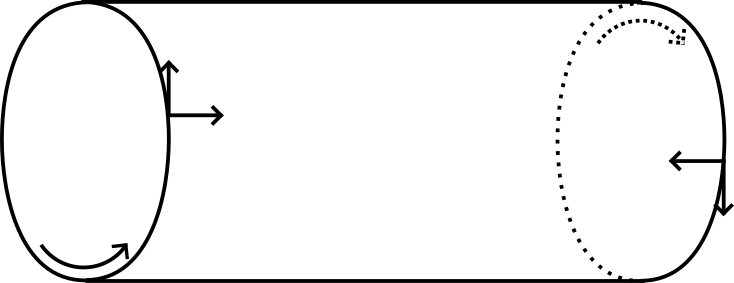
\includegraphics[width=.6\textwidth]{img/cyl.png}
    \caption{The cylinder $S^1\times [0,1]$ with boundary orientations induced by the inner normal direction.}\label{fig:cyl}
\end{figure}
Both boundary components of the cylinder are a circle, which we consider a $\BSO\to\BO$-manifold for this example. 
Picking the outer normal to induce the boundary orientations would have exactly switched the induced orientations on the two circles.\\
There is another subtle phenomenon which is illuminated by this cylinder:
Note how picking the inwards normal direction on both sides induces different orientations on the two circles.
If we were to define a bordism $M\bord M^\prime$ na\"{i}vely as a manifold with boundary $M\amalg M^\prime$, the resulting equivalence relation would have no reason to be reflexive, as the cylinder $M\times [0,1]$ in the oriented case would not define a bordism $M\bord M$.
This subtlety leads to the following defininition, artificially fixing the reflexivity problem.
\begin{defi}[Opposite manifold]
    Let $M\times[0,1]$ be a $\t$-Manifold. Then we call $M\times\{1\}$ and $M\times\{0\}$ with the induced boundary $\t$-structures opposites, and denote $M\times\{1\}$ with $-M\times\{0\}$ and vice versa. 
\end{defi}
By the path lifting property for fibrations, any $\t$-structure on $M\cong M\times\{0\}$ determines uniquely a $\t$-structure on $M\times[0,1]$, so every $\t$-manifold $M$ has an opposite $-M$.
As an example, again look at \fref{fig:cyl}, to see that as $\BSO \to \BO$-manifolds the opposite of $S^1$ oriented counterclockwise is $S^1$ oriented clockwise.
Moreover, we can forget orientation and see that as $\id_\BO$-manifolds the opposite of $S^1$, or any manifold for that sake, is just $S^1$.
\begin{defi}[$\t$-bordism]
    Let $M,M^\prime$ be two closed $\t$-Manifolds of dimension $d-1$. A $\t$-bordism $W\colon M\bord M^\prime$ consists of a $d$-dimensional $\t$-manifold $W$ together with a $\t$-preserving diffeomorphism $\partial W \cong M\amalg -M^\prime$.
\end{defi}
If $M$ and $M^\prime$ are diffeomorphic by a $\t$-preserving diffeomorphism $\phi\colon M\to M^\prime$, then they are also $\t$-bordant, as the cylinder $M^\prime \times [0,1]$ has boundary $M\amalg -M$ which by $\phi^{-1}\amalg \id_{-M}$ is diffeomorphic to $M^\prime\amalg -M$ preserving $\t$-structure.
This suggests we should think of bordism as a weakening of diffeomorphism, and motivates to show
\begin{thesisprop}
    The relation 
    \begin{equation*}
        M \sim M^\prime \:\Leftrightarrow\:\exists\:\t\text{-bordism }W\colon M\bord M^\prime
    \end{equation*}
    is an equivalence relation on the set of all closed $d$-dimensional $\t$-manifolds.
\end{thesisprop}
\prf
For reflexivity, consider the $\t$-manifold $W = M\times [0,1]$. 
By definition of the opposite, it has boundary $M\amalg -M$, and thus defines a $\t$-bordism $W\colon M\bord M$.
Let $W\colon M\bord M^\prime$ now be any $\t$-bordism, then $-W$ defines a $\t$-bordism $M^\prime \bord M$, as $\partial (- W) = -\partial W = M^\prime \amalg -M$, proving symmetry of the relation.
This comes with the caveat of $-W$ not being properly defined by us as $W\times[0,1]$ is a manifold with corners and not only boundary, and also misses any justification for the equality $\partial (-W) = -\partial W$.
The latter is easily seen to be true as $\partial W \times [0,1]\hookrightarrow W\times[0,1]$ has boundary $\partial W \amalg -\partial W$, the former becomes welldefined as one defines a notion of manifolds with corners.
Therefore we shall not digress further and discuss transitivity:\\
Let $W\colon M^\prime \bord M$ and $W^\prime \colon M \bord M^{\prime\prime}$ be $\t$-bordisms. 
We claim that by gluing togeter $W^{\prime\prime} = W\cup_{M} W^\prime$ we get a $\t$-bordism $M^\prime\bord M^{\prime\prime}$.
The critical part is the $\t$-structure on $W^{\prime\prime}$.
Begin by using compactness of $M$ to choose a closed collar neighbourhood of $-M$ as $M\times\{\varepsilon\}$ in $M\times[0,\varepsilon]\subset W$.
The $\t$-structure induced on $M\times[0,\varepsilon]$ by the restriction from $W$ agrees with the cylinder $\t$-structure given by the right lifting property against $M\times\{\varepsilon\} \hookrightarrow M\times[0,\varepsilon]$ as both induce the $-M$ structure on $M\times\{\varepsilon\}$.
Similarly, choose a collar neighbourhood of $M$ as $M\times\{0\}$ in $M\times[0,\delta]\subset W^\prime$ with induced $\t$-structure.
The diffeomorphism 
\begin{equation*}
    \phi\colon M\times[0,\varepsilon] \to M\times[0,\delta],\quad (x,t)\mapsto \left(x,\delta -\frac{\delta}{\varepsilon}t\right)
\end{equation*}
preserves $\t$-structure, as it sends the inner normal direction of $M\times\{\varepsilon\}$ in $M\times[0,\varepsilon]$ to the inner normal direction of $M\times\{0\}$ in $M\times[0,\delta]$.
Therefore the gluing $W^{\prime\prime} = W \cup_\phi W^\prime$ gives the desired $\t$-manifold with boundary $M^\prime\amalg -M^{\prime\prime}$
\endprf
The disjoint union $\amalg$ equips the set of all $\t$-preserving diffeomorphism classes of $d$-dimensional $\t$-manifolds with the structure of an associative magma.
Furthermore, the disjoint union behaves well around bordisms, since taking the boundary distributes over $\amalg$.
The structure thus descends, making
\begin{equation*}
    \Omega_d^\theta = \big\{\text{closed } d\text{-dimensional } \t\text{-manifolds}\big\}/_{\text{bordism } \sim}
\end{equation*}
an Abelian semigroup with neutral element given by the class of the empty manifold $[\emptyset]$, viewed a manifold of dimension $d$.
If one does not like to fiddle with the empty manifold, let it be noted that for any $\t$, the disk $D^n$ admits a $\t$-structure as it is contractible, and thus the sphere $S^{n-1} = \partial D^n$ inherits a boundary $\t$-structure such that $[S^{n-1}] = [\emptyset]$ can be taken as a neutral element instead.
A shift in perspective makes the cylinder $M\times [0,1]$ a $\t$-bordism $M\amalg (-M) \bord \emptyset$, so we have inverses in the semigroup given by the opposite manifolds.
\begin{defi}[Bordism group]
    The $\t$-bordism group is the abelian graded group
    \begin{equation*}
        \Omega_\ast^\t = \left( \bigcup_{d\in\N} \Omega_d^\t, \amalg, [\emptyset] \right)
    \end{equation*}
    of all closed $\t$-manifolds up to $\t$-bordism.
\end{defi}
Recall, that $\BO$ has an $H$-space structure $\oplus\colon\BO \times \BO \to \BO$ coming from the Whitney-sum of vectorbundles. 
Whenever we have such an $H$-space structure on $B$ and $\t$, such that the diagram
\begin{center}
\begin{tikzcd}
    B \times B \arrow[r]\arrow[d,"\t\times\t"] & B\arrow[d,"\t"]\\
    \BO\times\BO \arrow[r,"\oplus"] & \BO
\end{tikzcd}
\end{center}
commutes, we may define a product on $\Omega_\ast^\t$:
Given $\t$-manifolds $M,M^\prime$, a $\t$ structure on $M\times M^\prime$ is given by the composition 
\begin{equation*}
    M\times M^\prime \overset{\hat\st \times \hat\st^\prime}{\longrightarrow} B\times B \to B
\end{equation*}
which is well defined, as $T(M\times M^\prime) \cong TM\oplus TM^\prime$.
Let $W\colon M\bord M^\prime$ be a $\t$-bordism and $N$ a closed $\t$-manifold.
Then $\partial (W\times N) = (\partial W)\times N$, thus $W\times N$ is a $\t$-bordism $M\times N\bord M^\prime\times N$.
Hence the product descends to bordism classes.
Since the one point manifold $\{\ast\}$ is a $\t$-manifold for any $\t$, such a product will always be unital.
It is furthermore associative, commutative and distributes over $\amalg$ up to $\t$-preserving diffeomorphism.
We conclude
\begin{thesisprop}
    For the tangential structures $\BSpin,\BSO$ and $\BO$ from the Whitehead-tower of $\BO$, we have a commutative, unital, graded ring
    \begin{equation*}
        \Omega_\ast^\t = \left( \bigcup_{d\in\N} \Omega_d^\t, \amalg, \times , [\emptyset], [\{\ast\}] \right)
    \end{equation*}
    of closed $\t$-manifolds up to $\t$-bordism.
\end{thesisprop}
\prf
The Whitney-sum of two orientable bundles is again orientable, and the Whitney-sum of two spinnable bundles is again spinnable, as one sees computing the Stiefel--Whitney-classes via the Whitney--product theorem.
This gives the according $H$-space structures, so the above applies.
\endprf
Before we study one of those rings, the unoriented bordism ring $\NN_\ast = \Omega_\ast^{\id_\BO}$ in excessive detail, let us first introduce an important class of examples of bordisms, the so called surgeries.
They rely solely on the observation that both $A = S^p\times D^q$ and $B = D^{p+1}\times S^{q-1}$ have boundary $S^p\times S^{q-1}$.
An occurance of either $A$ or $B$ embedded in a manifold may thus be cut out and replaced by the other.
\begin{defi}[Surgery]
    Given a $d$-dimensional manifold $M$ and an embedding $\iota\colon S^p\times D^q \hookrightarrow M$ for $p+q=d$, we say the manifold
        \begin{equation*}
            \quotient{\big(M \setminus \iota(S^p\times\{0\})\big) \amalg D^{p+1}\times S^{q-1}}{\iota(x,ty) \sim (tx,y) \text{ for all } (x,y)\in S^p\times S^{q-1}, t\in[0,1]}
        \end{equation*}
    is \emph{obtained} from $M$ by a dimension $p$ (or codimension $q$) surgery.
\end{defi}
The easiest example to visualize is the codimension $n$ surgery in an $n$-dimensional manifold $M$.
Take an embedding $S^0\times D^n \hookrightarrow M$, that is just two copies of $D^n$.
Now puncture each of the copies of $D^n$ and obtain two embedded $D^n\setminus \{0\}$.
Introduce the $t$-coordinate from the definition by deforming each punctured disk $D^n\setminus\{0\}$ to a neck $S^{n-1}\times (0,1]$.
As $S^0 = \{\pm 1\}$, our equivalence relation identifies an embedded point of one of the necks $(\pm 1, x, t) \in S^0\times S^{n-1}\times (0,1]$ with a point of the cylinder $(\pm t, x) \in D^1\times S^{n-1}$.
One should imagine gluing the two necks onto a cylinder from opposite directions, therefore resulting in a tube $S^{n-1}\times D^1$ connecting the two embedded copies $\{\pm 1\}\times S^{n-1}$.
If $M = N \amalg N^\prime$ for two connected $n$ dimensional manifolds $N,N^\prime$, embedding $\{1\}\times D^n$ in $N$ and $\{-1\}\times D^n$ in $N^\prime$ and then performing the described surgery on $S^0\times D^n$, one obtains a manifold known as the connected sum $N\connsum N^\prime$.
We depict a connected sum in \fref{fig:connsum} for consideration of the above described process.
\begin{figure}
    \centering
    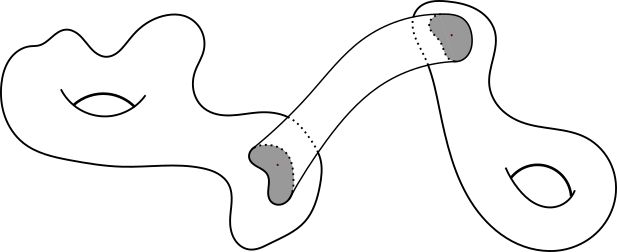
\includegraphics[width=.8\textwidth]{img/connsum.png}
    \caption{A connected sum of two manifolds. The gray areas are the embedded disks, on which the surgery is performed}\label{fig:connsum}
\end{figure}
The connection of surgeries to bordism is established in:
\begin{thesisprop}
    If $M^\prime$ is obtained from $M$ via a surgery, $[M] \equiv [M^\prime]$ in $\Omega_\ast^{\id_\BO}$.
\end{thesisprop}
\prf
Let $\iota\colon S^p \times D^q \hookrightarrow M$ be the embedding of the surgery move turning $M$ into $M^\prime$.
The so called \emph{trace} of the surgery is the space
\begin{equation*}
    W = \quotient{(M \times [0,1]) \amalg (D^{p+1}\times D^q)}{(\iota(x),1) \sim x \text{ for all } x\in S^p\times D^q \subset D^{+1}\times D^q},
\end{equation*}
which by writing it as the gluing $W = (M\times[0,1])\cup_{(\iota ,1)} (D^{p+1}\times D^q)$ is a manifold.
The boundary of this manifold is given by $M\cong M\times\{0\}$ on the one side and the surgery result $M^\prime$ on the other.
\endprf
A choice of $\t$-structures on $S^p\times D^q$ and $D^{q+1}\times S^{q-1}$ that induce the same boundary $\t$-structure on $S^p\times S^{q-1}$ allows for a well defined notion of $\t$-surgery, where one requires the embedding $\iota$ to be $\t$-preserving.
If moreover these compatible $\t$-structures on $S^p\times D^q$ and $D^{p+1}\times S^{q-1}$ are induced as the boundary $\t$-structures of a common $\t$-structure on $D^{p+1}\times D^q$, one can produce a more careful gluing of the trace, and obtain a version of the above proposition for $\t$-surgeries and $\t$-bordism.
This more careful approach can be read about in \cite{milnor:surg}, where everything is done for $\t\colon \BSO \to \BO$, but the arguments all apply to the sketched general case above.
It then turns out, that bordism and surgery are even closer related than above proposition indicates, one can for example prove statements like:
\begin{thesislemma}[thm.~1 in \cite{milnor:surg}]
    A $d$ dimensional manifold $M^\prime$ can be obtained from a $d$ dimensional manifold $M$ via a sequence of oriented surgery moves if and only if $[M] \equiv [M^\prime]$ in $\Omega_d^\BSO$.
\end{thesislemma}
Because of this lemma, we may switch the group operation in the groups $\Omega_\ast^{\BSO\to\BO}$ and $\Omega_\ast^{\id_\BO}$ away from the disjoint union $\amalg$ to the connected sum $\connsum$.
Thus, working in the unoriented bordism group, we may without loss of generality assume all representatives to be connected manifolds.
This justifies our assumption of connectedness in the rest of this thesis.

